{
\newcommand\myrect[5]{\draw (#1,#2) rectangle ({#1+#3},{#2+#4}) node[pos=0.5] {#5} ; }
\newcommand\minicipher[3]{
	\myrect{#1}{#2}{1}{1}{#3}
    \draw (#1+1, #2+0.3) -- (#1+1-0.15, #2+0.5) -- (#1+1, #2+1-0.3) ;
}

\begin{figure}
  \centering
%   \begin{comment}
%   \begin{subfigure}[t]{0.15\textwidth}
%     \centering
%     \begin{tikzpicture}[xscale=0.8, yscale=-0.5]
%     	\minicipher{-1.5}{-2}{$T^{-1}$}
%     	% left input to T
%         \draw [->] (-1,-2) -- (-1,-3);
%     	% right parallel
%     	\draw [->] (0.5,0) -- (0.5,-3);
%         % T to out left
%         \draw [->] (-1,0) -- (-1,-1);
%     	% right out to T key
%     	\draw [->] (0.5,-1.5) -- (-0.5,-1.5);
%     \end{tikzpicture}
%     \caption{Initial structure.}
%   \end{subfigure}
%   \end{comment}
  \begin{subfigure}[t]{0.25\textwidth}
    \centering
    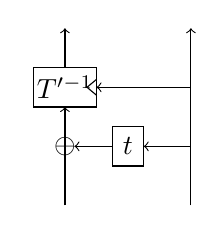
\begin{tikzpicture}[xscale=0.8, yscale=-0.5]
        \minicipher{-1.5}{-2}{$T'^{-1}$}
    	\myrect{-0.25}{-0.5}{0.5}{1}{$t$}
    
    	% left input to T
        \draw [->] (-1,-2) -- (-1,-3);
    	% right parallel
    	\draw [->] (1,1.5) -- (1,-3);
        % T to out left
        \draw [->] (-1,1.5) -- (-1,-1);
    	% right out to T key
    	\draw [->] (1,-1.5) -- (-0.5,-1.5);
    	% right to t
    	\draw [->] (1,0) -- (0.25,0);
    	% t to xor
    	\draw [->] (-0.25,0) -- (-0.85,0);
    	\draw (-1.0,0) node[inner sep=0](xor){$\oplus$} ;
    \end{tikzpicture}
    \FigDef{simplify-t-a}{Detaching a linear Feistel round.}
  \end{subfigure}
  \hspace{0.3cm}
  \begin{subfigure}[t]{0.32\textwidth}
    \centering
    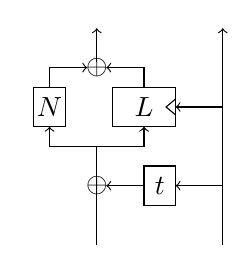
\begin{tikzpicture}[xscale=0.8, yscale=-0.5]
    	\minicipher{-0.75}{-2.5}{$L$}
    	\myrect{-0.25}{-0.5}{0.5}{1}{$t$}
    	\myrect{-2}{-2.5}{0.5}{1}{$N$}
    
    	% right parallel
    	\draw [->] (1,1.5) -- (1,-4);
    
        % left bot to L and N
        \draw [->] (-1,1.5) -- (-1,-1) -- (-0.25,-1) -- (-0.25,-1.5);
        \draw [->]             (-1,-1) -- (-1.75,-1) -- (-1.75,-1.5);
    
    	% N and L to top
        \draw [->] (-1.75,-2.5) -- (-1.75,-3) -- (-1.15,-3);
        \draw [->] (-0.25,-2.5) -- (-0.25,-3) -- (-0.85,-3);
    
    	% xor
    	\draw (-1.0,-3) node[inner sep=0](xor){$\oplus$} ;
    
    	% xor to top
    	\draw [->] (-1.0,-3.15) -- (-1.0,-4);
    
    	% right out to T key
    	\draw [->] (1,-2) -- (0.25,-2);
    	% right to t
    	\draw [->] (1,0) -- (0.25,0);
    	% t to xor
    	\draw [->] (-0.25,0) -- (-0.85,0);
    	\draw (-1.0,0) node[inner sep=0](xor){$\oplus$} ;
    
    \end{tikzpicture}
    \FigDef{simplify-t-b}{Splitting $T'^{-1}$ into $N$ and $L$.}
  \end{subfigure}
  \hspace{0.3cm}
  \begin{subfigure}[t]{0.32\textwidth}
    \centering
      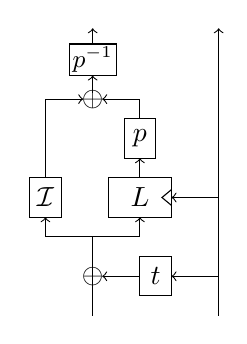
\begin{tikzpicture}[xscale=0.8, yscale=-0.5]
    	\minicipher{-0.75}{-2.5}{$L$}
    	\myrect{-0.25}{-0.5}{0.5}{1}{$t$}
    	\myrect{-2}{-2.5}{0.5}{1}{$\mathcal{I}$}
    	\myrect{-0.5}{-4}{0.5}{1}{$p$}
    	\myrect{-1.375}{-5.9}{0.75}{0.8}{\small $p^{-1}$}
    
    	% right parallel
    	\draw [->] (1,1.0) -- (1,-6.3);
    
        % left bot to L and I
        \draw [->] (-1,1.0) -- (-1,-1) -- (-0.25,-1) -- (-0.25,-1.5);
        \draw [->]             (-1,-1) -- (-1.75,-1) -- (-1.75,-1.5);
    
    	% L to p
        \draw [->] (-0.25,-2.5) -- (-0.25,-3);
    
    	% I and p to top
        \draw [->] (-1.75,-2.5) -- (-1.75,-4.5) -- (-1.15,-4.5);
        \draw [->] (-0.25,-4) -- (-0.25,-4.5) -- (-0.85,-4.5);
    
    	% xor
    	\draw (-1.0,-4.5) node[inner sep=0](xor){$\oplus$} ;
    
    	% xor to p^-1
    	\draw [->] (-1.0,-4.65) -- (-1.0,-5.1);
    
    	% p^-1 to top
    	\draw [->] (-1.0,-5.9) -- (-1.0,-6.3);
    
    	% right out to T key
    	\draw [->] (1,-2) -- (0.25,-2);
    	% right to t
    	\draw [->] (1,0) -- (0.25,0);
    	% t to xor
    	\draw [->] (-0.25,0) -- (-0.85,0);
    	\draw (-1.0,0) node[inner sep=0](xor){$\oplus$} ;
      \end{tikzpicture}
    \FigDef{simplify-t-c}{Simplifying $N$ into $\mathcal{I}$ and linear functions.}
  \end{subfigure}
  \FigDef{simplify-t}{Simplifying the keyed permutation $T'^{-1}$.}
\end{figure}

}